\documentclass[runningheads,a4paper]{llncs}

\usepackage{amssymb}
\usepackage{graphicx}
%\usepackage{multirow}
\usepackage{url}
\usepackage{color}

\urldef{\mailthu}\path|{lijuanzi@}tsinghua.edu.cn|
\newcommand{\keywords}[1]{\par\addvspace\baselineskip\noindent\keywordname\enspace\ignorespaces#1}
\newcommand{\para}[1]{\vspace{0.1cm}\noindent\textbf{#1}}

\begin{document}
\mainmatter

\title{Building Large-Scale Bilingual Knowledge Base from Multi-Encyclopedia}
\titlerunning{Bilingual Knowledge Base}
\author{Mingyang Li$^\dag$ \and Yao Shi$^\dag$ \and Zhigang Wang$^\dag$}
\authorrunning{Mingyang Li et.al}

\institute{$^\dag$Tsinghua National Laboratory for Information Science and Technology,\\
Department of Computer Science and Technology,\\
Tsinghua University, Beijing 100084, China\\
\mailthu\\
}

\maketitle

\begin{abstract}
    Abstract Text

\keywords{Knowledge Base, Semantic Web, Linked Data, Ontology, Cross-lingual}
\end{abstract}

\section{Introduction}

Introduction Text

Current situation of KB
Current situation of cross-lingual KB 

Knowledge bases such as DBpedia, YAGO, and BabelNet are mainly built upon the multilingual Wikipedia. ..

Some problems are to be addressed:
\begin{itemize}
  \item The imbalanced size of different Wikipedia languages leads to less data of various languages, which makes it more difficult to build a multi-language knowledge base.
  \item The number of existed cross-lingual links in Wikipedia is so small that affects the quality of a bilingual knowledge base. Especially there is no obvious links in properties.
  \item The large but irrigorous category system in Wikipedia causes incorrect semantic relations in taxonomy. For example, 
\end{itemize}

Our main contributions include:
\begin{itemize}
  \item We propose a method to build a Chinese-English ontology combining four encyclopedias, which are English Wikipedia, Chinese Wikipedia, Baidu and Hudong. The latter three contain large amount of Chinese knowledge, which helps balance information of two languages and enrich the knowledge base.
  \item We extend the cross-lingual link set by employing a cross-lingual knowledge linking discovery approach for concept and instance, and by analysing templates in Wikipedia for property.
  \item We prune the original taxonomy, which is extracted from encyclopedia category system, to retrieve more precise SubClassOf and InstanceOf relation.
  \item A website is developed based on our ontology and also a SPARQL interface is provided for public query operations in our knowledge base.
\end{itemize}

The rest of the paper is organized as follows. Section \ref{sec:pre} introduces the four encyclopedias which are English Wikipedia, Chinese Wikipedia, Baidu and Hudong. Besides, definitions are proposed in this section. Section \ref{sec:oe} presents the extraction approach in concept, instance and property level. Method of initiating cross-lingual link set will also be mentioned. Section \ref{sec:cle} propose an extension approach for discovering more cross-lingual relations. Section \ref{sec:tp} describes how to prune the taxonomy. Section \ref{sec:result} shows the results of established knowledge base. Section \ref{sec:con} gives the conclusion and future work.

\section{Preliminary}
\label{sec:pre}
In this section, we firstly introduce the four encyclopedias which are used to build and enrich our knowledge base. They are English and Chinese Wikipedia, Baidu and Hudong Encyclopedia. Then we gives some related definitions to formalize our model.

\subsection{Encyclopedias}
\label{sec:encyclopedias}
\subsubsection{Wikipedia}
Nowadays, Wikipedia is the largest store of human knowledge. It was launched in 2001 and has hold over 35 million articles in 288 language by 2015. Among these articles, English articles contribute most. There are \textcolor{red}{4,867,719} articles in English while only \textcolor{red}{over 800,000 articles} in Chinese. It is obvious that the quantity of English articles is far more than Chinese. Such imbalance makes those ontologies based on Wikipedia only behave bad in cross-lingual aspect. For example, DBpedia has 683 concepts in English while only 11 Chinese concepts, that helps little when other poeple want to do cross-lingual research depending on DBpedia. To avoid the imbalance problem, two other Chinese encyclopedias are utilized to enrich Chinese source.
Articles in Wikipedia are manually editted by various authors. Wikipedia provides many templates to guide authors composing their context in a regular way. For example, \textcolor{red}{China use template XXX}. Moreover, an infobox in one article also follows an infobox template, which maintains a property set of similar articles and display labels on website page.
\subsubsection{Other Chinese Encyclopedias}
There are several large-scale monolingual Chinese Encyclopedias currently. Among those, Baidu Baike and Hudong are the most well-known. Hudong was founded in 2005 and contains more than 12 millions articles with about 9 millions experts' contribution util 2015, April. At the mean time, Baidu Baike maintains more than 11 millions articles. These two resource are similar in article structure, somethimes even in content. 
\subsubsection{Encyclopedia Page}
All these four encyclopedias have two important elements, articles and category taxonomy. A taxonomy presents the relation between categories. Usually a category has its sub classes and super classes. Besides, an article belongs to one or more categories. Fig. \ref{fig:hudong-taxonomy} An article describes an topic with rich information created and modified by several verified editors. The content and relation of an article provide a lot when building a \textcolor{red}{global?} knowledge base. In general, there are five elements can be exploited:
\begin{figure}
    \centering
    %\subfigure[]{
    \begin{minipage}[t]{0.5\textwidth}
        \centerline{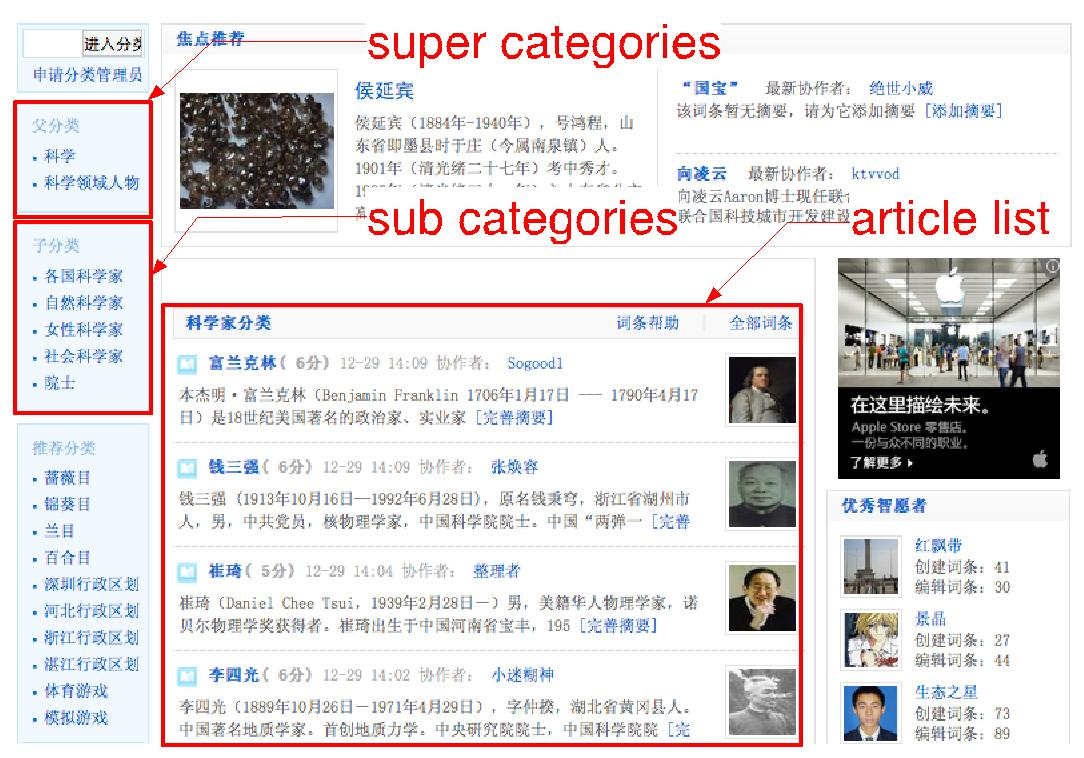
\includegraphics[width=0.8\columnwidth]{fig/hudong-taxonomy}}
        \label{fig:hudong-taxonomy}
        \caption{Taxonomy in Hudong.}
    %}
    \end{minipage}%
    \begin{minipage}[t]{0.5\textwidth}
        \centerline{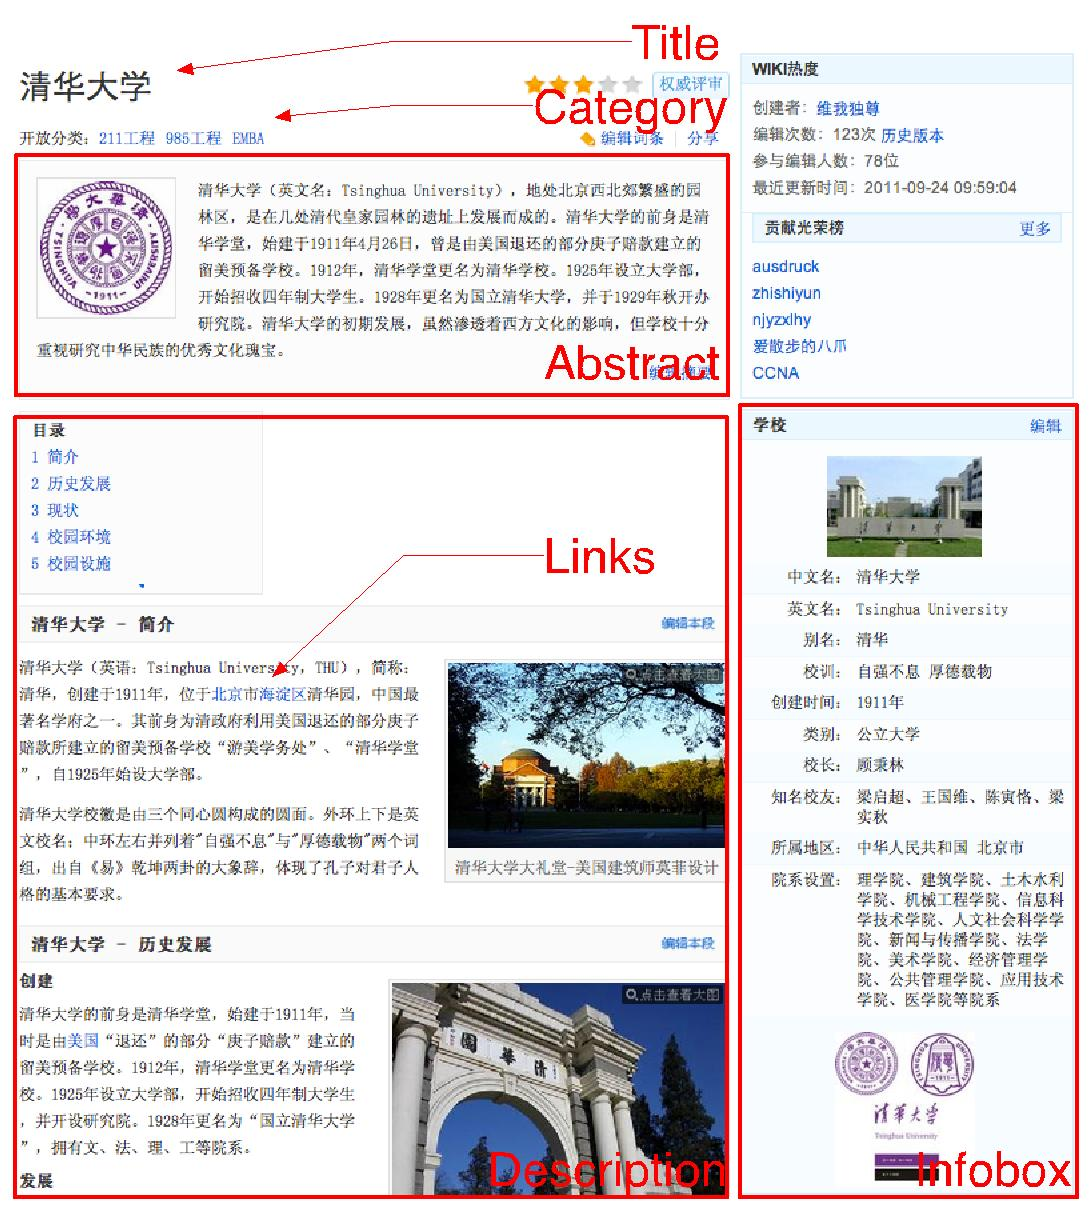
\includegraphics[width=0.8\columnwidth]{fig/baidu-article}}
        \label{fig:baidu-article}
        \caption{A snap of an article in Baidu Baike}
    \end{minipage}%
\end{figure}
\begin{itemize}
  \item Title: A Title is the label of topic. Every article has a unique title, which can be used to distinguish each topic.
  \item Abstract: An abstract is a brief summarize of the article topic. It's always the first paragraph of an article. Usually it can be taken as an important feature to a topic. 
  \item Infobox: Most of articles contain infobox. An infobox maintains structured data which are in general subject-attribute-value triples formalized as a table. Information in this table includes important properties of the topic.
  \item Links: Links are entries directing to other articles within the encyclopedia. They lead readers to reference articles. Actually, they represent the relations between the current article and other articles.
  \item Category: The categories that an article belongs to are usually listed below the article page, shown as tags. An article attaches to one or more categories.
\end{itemize}
Fig. \ref{fig:baidu-article} shows a snap of an article in Baidu Baike. The five elements mentioned above are annotated.
\subsection{Cross-lingual Links}
In order to build a bilingual knowledge base, we need the relation between Chinese source and English source, which helps merge different language information into their unique and common topic. In Wikipedia, most articles have language links which guide the reader to the article in specific language under the same topic. Fig. \ref{fig:lang-link} shows an example of language links in Wikipedia. Taking advantage of such existed links in Wikipedia, we can generate an initial bilingual ontology based on Chinese and English Wikipedia. However, the result is just an ontology based on Wikipedia, like DBpedia. To combine Hudong and Baidu Baike ,which are lack of cross-lingual information but more Chinese source, we employ the approach from \cite{} to discover bilingual links between English Wikipedia and Hudong in Section \ref{sec:cld}  

\subsection{Definitions}

\section{Extraction}
\label{sec:oe}
In order to build a billinual knowledge base, we first set up an ontology to schema information from the four encyclopedia. The ontology includes concepts, which are extracted from category taxonomy, instances, which are defined according to articles and properties, which are based on infobox and also templates assistant. We will describe our building approach as follow.
\subsection{Concept Extraction}
\label{sec:ce}
A concept in ontology is defined as a type of similar instances. For example, the concept of instance \emph{Tsinghua University} is \emph{University} or \emph{Organization}. In general, a concept has super classes and sub classes, which means it has \emph{subClassOf} relation with other classes. Those concepts comprise a taxonomy which presents a backbone of the ontology.
In an encyclopedia, a category groups several articles and also has super-categories and sub-categories, just like concept doing. Therefore we can extract concepts based on existed category system. 
However, the whole taxonomy can not directly transform from category system because of the following problems:
\begin{itemize}
    \item There are auxiliary categories in Wikipedia, which help arrange specific articles or category pages that are typical of Wikipedia. For example, \textcolor{red}{list of ... or tempalte:infobox}
    \item Some sub-category links in the category system maybe inconsistent. Some categories may contain itself as sub-category, or contain sub-category that also be the super-category of it. As Fig. \ref{fig:category-mistakes} shows: In Hudong, the sub-categories of 国家元首(Head of State) contains itself as a child, which causes a circle in taxonomy tree. Meanwhile, in Wikipedia, \textcolor{red}{例子}
    \item Some categories relate to only one or two articles. According to the definition of concept, such categories are less representive to a group of instance, therefore it's unwise to retain it as concept.
\end{itemize}
   To retrieve a cleaner and preciser concept taxonomy, we firstly do some refine works as follow:
\begin{itemize}
    \item Delete specific categories in Wikipedia.
    \item Delete inconsistent sub-categories and keep the super one.
    \item Delete categories that relate to less than two articles.
\end{itemize}
The cleaning works are carried out in all encyclopedias for rule consistency when extracting. The remaining categories comprise an original concept taxonomy. A category and its sub-categories are correlated by the relation \emph{SubClassOf}, and a category and its articles are correlated by the relation \emph{InstanceOf}. However, there are still inaccurate samples in the two relations. For example, \textcolor{red}{example}. We will prune the taxonomy later.

\subsection{Property Extraction}
\label{sec:pe}
A property is defined as an attribute of instance. It represents the relation between two instances or an instance and its value. We divided properties into two types: datatype properties, which \textcolor{red}{...}; object properties, which \textcolor{red}{...}. Considering both content and infobox of an article, we extract two groups of properties, general-properties and Infobox-properties.

\subsubsection{General-properties}
Characteristics of an instance are seen as general-properties, including label, abstract, and url. Those properties describe specific information of an instance. The label property identifies a unique instance, whose value is article title. The abstract property provides a brief description of an instance, whose value is the first paragraph of article. The url property saves the resource of an instance, which is actually a url in Wikipedia or Hudong or Baidu Baike. All of them are datetype properies.
\subsubsection{Infobox-properties}
Attributes acquired from infobox data are considered as Infobox-properties, such as 上映时间(release date), 导演(directed by) in a movie's infobox. All attributes are relating with a typical value in the infobox, the value maybe a text or a reference, usually a url links to anothor instance. The type of a property, datatype or object, depends on the value. Ordinarily, a plain text value marks the property as datetype while an instance reference determines the property as object. For example, the attribute 上映时间(release date) can be defined as a datatype property as its value is a datetime string. Meanwhile, 导演(directed by) can be an object property because its value points to a person who directed the movie.
We occur some chanllenges when extracting properties from infoboxes:
\begin{itemize}
    \item There are some 
    \item 
    \item 
\end{itemize}

\subsection{Instance Extraction}
\label{sec:ie}
In encyclopedia, an article describes an unique entity in the world. Therefore we can extract article content as an instance. But we can't transform all the articles as instances because there are many illustrative or structure-related articles in Wikipedia, including Category List pages, Template documentations \textcolor{red}{and...}.
Each instance contains relations with concepts and properties. Take the movie 星际穿越(Interstellar) as an example in Fig.\ref{fig:interstellar}. concepts are assigned according to the category tags below the article page. 美国科幻片(American science fiction films) is a concept to Interstellar. In the meantime, we obtain label property from article title, which is 星际穿越(Interstellar) and abstract property from the first paragraph. Infobox-properties are also acquired via extracting from infobox in the article. Besides, according to links placing in content, we gain the reference between the current instance to others, such as 华纳兄弟(Warner Bros.).
After the preprocessing above, we harvest two types of information. One is the characteristics of instance, including instance-label, instance-abstract. The other is relationships, containing concept-instance, instance-property-value and instance-instance.
\subsection{Cross-lingual Links Extraction}
\label{sec:cld}
Wikipedia has \textcolor{red}{number} cross-lingual links between articles of English and Chinese. By extracting language links from Wikipedia, we can get an initial cross-lingual link set of concepts and instances. 
However, in property aspect, there is no obvious infobox links between English and its mapping Chinese article. According to the edit mechanism of Wikipedia, we use infobox template to get display label and cross-lingual links of an infobox-property. Fig. \ref{fig:template} shows a typical example of infobox template. 
\section{Cross-lingual Links Extension}
\label{sec:cle}
Research of Wang ZhiChun

After the extracting preprocessing, we acquire a series of semi-structured data, including concept information, property pairs, instance information, relations among the three and cross-lingual links. Holding these raw data in hand, we then build an ontology schema for the futher knowledge base.

\section{Cross-lingual Knowledge Base Building}
To construct an cross-lingual ontology schema with existing semi-structured data, firstly we link the four encyclopedia, which is to say, combining concept, instance and property of the four sources into one if it represents the same thing. Secondly, we prune the taxonomy which generates from concept relationships to retain a more accurate one. At last, we hung instances and properties on to taxonomy to create a complete knowledge base.

\subsection{Cross-lingual Linking}
\label{sec:cld}
combine four ontology into on

\subsection{Taxonomy Prune}
\label{sec:tp}
Research of Wang Zhigang

\subsection{Taxonomy Prune}


\section{Result}
\label{sec:result}
\subsection{DataSet}
The four encyclopedias and their statistics data
\subsection{Extracted Knowledge Base}
Xlore statistics data.
\subsection{Query Interface}
Xlore query interface 

\section{Related Work}
\label{sec:work}

\section{Conclusion and Future Work}
\label{sec:con}

\section*{Acknowledgement}
Thanks anonymous reviewers for their valuable suggestions that help us improve the quality of the paper. Thanks Prof. Chua Tat-Seng from National University of Singapore for discussion. The work is supported by 973 Program (No. 2014CB340504 ), NSFC-ANR (No. 61261130588), Tsinghua University Initiative Scientific Research Program (No. 20131089256) and THU-NUS NExT Co-Lab.

\bibliographystyle{splncs03}
\bibliography{paper}

\end{document}

